% The two-minute overview for the mid-evaluation: eight slides, then backup slides for questions.
% The words to say over each slide are in presentation.md. Built with xelatex (metropolis theme).
\documentclass[aspectratio=169,11pt]{beamer}
\usetheme[progressbar=frametitle,numbering=fraction]{metropolis}
\usepackage{booktabs}
\usepackage{tabularx}
\graphicspath{{../../diagrams/out/}{../mid-demo-report/}}
\setbeamertemplate{frame footer}{Exchange Student Guide · CS5013}
\setbeamerfont{footnote}{size=\tiny}
% One box of the slices slide: name, x, y, title, what it does.
\newcommand{\slicenode}[5]{\node[slice] (#1) at (#2,#3) {\textbf{#4}\\[-1pt]{\tiny #5}};}

\title{Exchange Student Guide}
\subtitle{A moderated, community-written knowledge base for exchange students at IIT Madras}
\author{Mikhail Novikov (GE26Z858) \and Abdirakhim Ismailov (GE26Z860)}
\institute{CS5013 Programming with AI · Mid-evaluation · Stakeholder: OGE, IIT Madras}
\date{October 2026}

\begin{document}
\maketitle

\begin{frame}{The problem, and who uses it}
\begin{columns}[T]
\column{0.5\textwidth}
\small
The information exists, but it is scattered across the IITM site, WhatsApp groups and blogs; a
student three days off the plane cannot find it.
\begin{itemize}
\item \alert{Student reads}: search, articles linked with \texttt{[[Title]]}, tags
\item \alert{Student writes}, with no account: a new article or an edit, with a photo
\item \alert{OGE moderates}: nothing is public until a moderator approves it
\end{itemize}
\vspace{0.4em}
39 starter articles from OGE's Handbook 2026.
\column{0.5\textwidth}
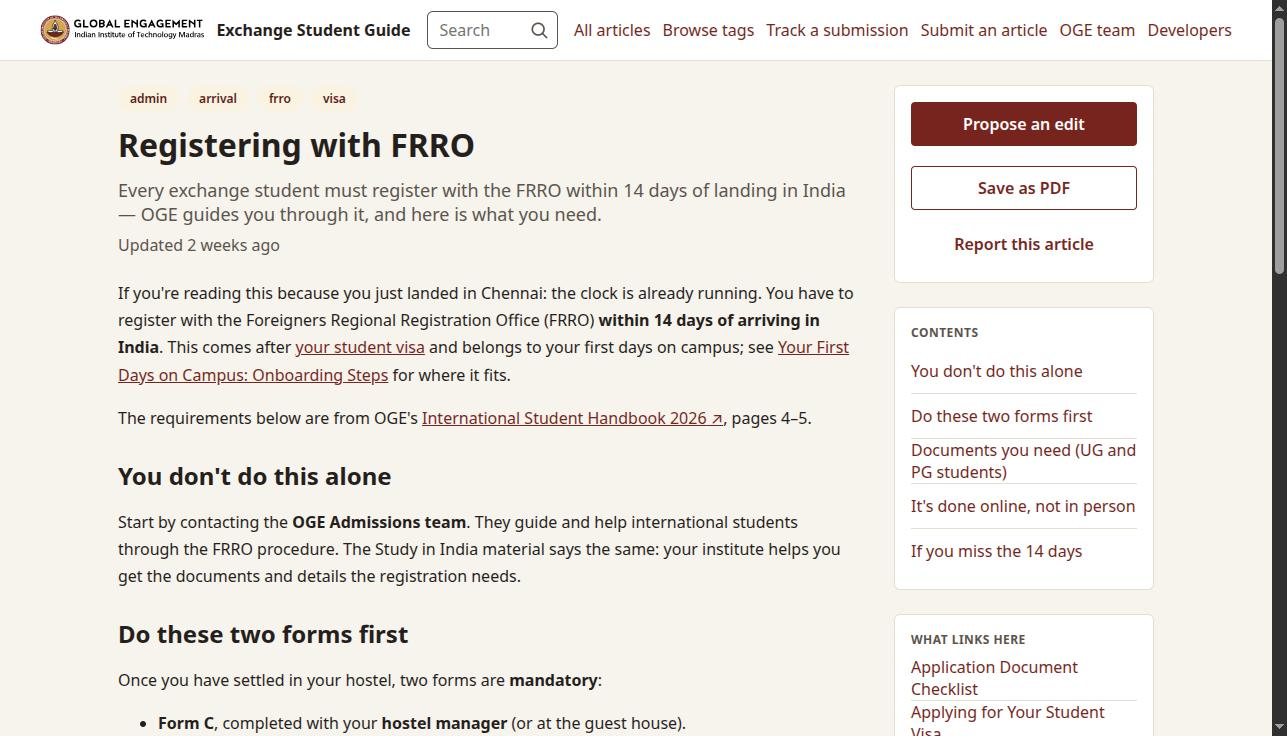
\includegraphics[width=\linewidth]{3-article.jpg}
\end{columns}
\end{frame}

\begin{frame}{Architecture: one process, three stores}
\begin{columns}[c]
\column{0.5\textwidth}
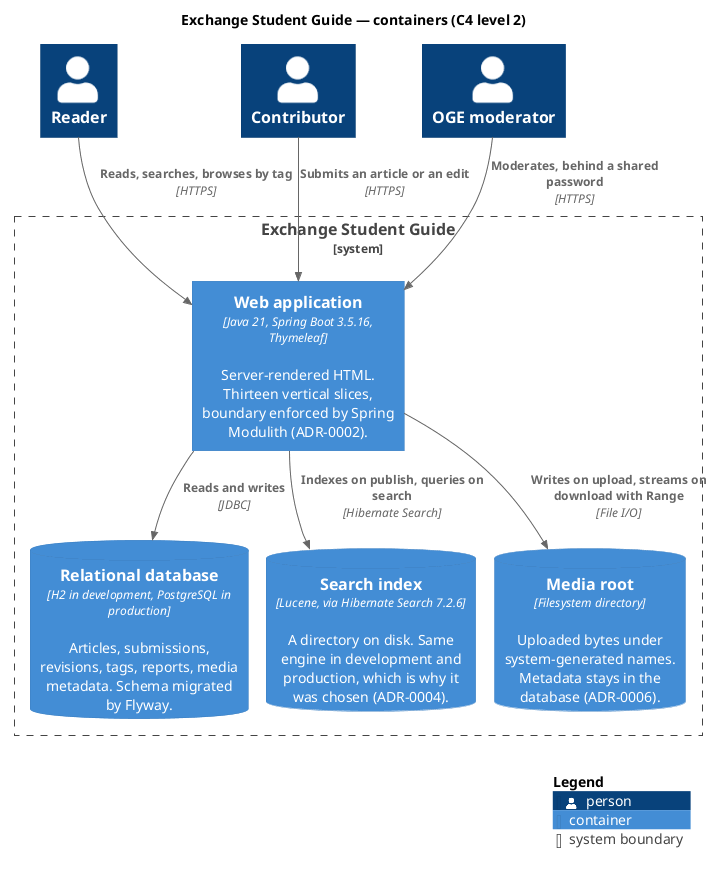
\includegraphics[width=\linewidth,height=0.78\textheight,keepaspectratio]{c4-container.png}
\column{0.5\textwidth}
\small
\begin{itemize}
\item \alert{Spring Boot 3.5, Java 21}, server-rendered Thymeleaf --- a modular monolith, not
  microservices: one team of two, one server at OGE
\item \alert{PostgreSQL} with Flyway: articles, every earlier version, submissions, tags, reports
\item \alert{Lucene} through Hibernate Search: same engine in tests and production; rebuilt at
  every start
\item \alert{Media root}: uploaded bytes on disk, metadata in the database
\item Runs with \texttt{docker compose up}
\end{itemize}
\end{columns}
\end{frame}

\begin{frame}{Thirteen slices, and a boundary the build enforces}
\centering
\begin{tikzpicture}[
  slice/.style={fill=mDarkTeal!8,rounded corners=2pt,minimum width=2.9cm,minimum height=0.72cm,
    font=\footnotesize,align=center},
  group/.style={font=\small\bfseries,text=mDarkTeal},
  every node/.append style={inner sep=2pt}]
  \foreach \x/\name in {0/Reading,3.7/Contributing,7.4/Moderating,11.1/Shared and support}
    \node[group] at (\x,0.75) {\name};
  \slicenode{home}{0}{0}{home}{pinned, recent, tags}
  \slicenode{articleview}{0}{-0.9}{articleview}{article, media, what links here}
  \slicenode{search}{0}{-1.8}{search}{Lucene, a marked passage}
  \slicenode{taxonomy}{0}{-2.7}{taxonomy}{the only writer of tags}
  \slicenode{contribute}{3.7}{0}{contribute}{form, checks, a number}
  \slicenode{media}{3.7}{-0.9}{media}{photo re-encoded, PDF, video}
  \slicenode{report}{3.7}{-1.8}{report}{a reader flags a problem}
  \slicenode{moderate}{7.4}{0}{moderate}{queue, diff, approve, pin}
  \slicenode{wikilink}{11.1}{0}{wikilink}{plain Java: [[Title]] → link}
  \slicenode{backlink}{11.1}{-0.9}{backlink}{the links table}
  \slicenode{shared}{11.1}{-1.8}{shared}{entities, login, CSP, limits}
  \slicenode{backup}{11.1}{-2.7}{backup}{export, import, seed}
  \slicenode{about}{7.4}{-2.7}{about}{OGE and developers pages}
  \draw[-latex,thick,mDarkTeal] (moderate) -- node[above,font=\tiny]{same checks} (contribute);
  \draw[-latex,thick,mLightBrown] (moderate.south) |- node[pos=0.75,below,font=\tiny,text=mLightBrown]
    {ArticleTextChanged (event)} (backlink.west);
\end{tikzpicture}

\vspace{0.5em}
\small
Inside every slice: root = \alert{published types} · \texttt{web/} controllers · \texttt{internal/}
services · \texttt{persistence/} repositories.\\
Another slice may use only the root, or an \alert{event}; \texttt{ModularityTest} (Spring Modulith)
and ArchUnit fail the build otherwise.
\end{frame}

\begin{frame}{Data flow: an edit, from the student to the live article}
\small
\begin{tabularx}{\textwidth}{@{}lX@{}}
\toprule
\textbf{1. contribute} & form → rate limit (5/hour) → \texttt{SubmissionService.check} → a
\texttt{Submission} row, tags, photo re-encoded → number \texttt{SUB-…}; the article is unchanged \\
\textbf{2. moderate} & queue → diff of the text as it reads (\texttt{TextDiff}) → approve or reject
with a reason \\
\textbf{3. approve} & old text kept as a \texttt{Revision} → \texttt{Article} updated → media moved →
event \texttt{ArticleTextChanged} \\
\textbf{4. after commit} & \texttt{backlink} re-reads the links; Hibernate Search updates the index
--- the change is live and searchable \\
\bottomrule
\end{tabularx}
\vspace{0.6em}

Every request has the same shape: \alert{route → \texttt{web/} controller → \texttt{internal/}
service → \texttt{persistence/} repository → Thymeleaf template}.
\end{frame}

\begin{frame}{What checks it}
\begin{columns}[T]
\column{0.5\textwidth}
\small
\begin{itemize}
\item \alert{649} application tests, \alert{356} for the tooling --- every push
\item The same suite on \alert{PostgreSQL 17} in CI
\item \alert{151} browser tests in Chromium with axe (accessibility), 320--1920\,px
\item \alert{Mutation testing}: 130 of 132 mutants killed
\item \alert{Property-based} tests: 1000 titles in English, Hindi, Tamil
\end{itemize}
\column{0.5\textwidth}
\small
\begin{itemize}
\item A test is red before the code exists
\item Test names are sentences:\\
  {\scriptsize\texttt{ten\_tags\_are\_accepted\_and\_}\\\texttt{eleven\_are\_refused}}
\item The demo rehearsal on Docker found 4 faults no unit test could see --- each fixed with the
  test that catches it
\end{itemize}
\end{columns}
\end{frame}

\begin{frame}{Written with AI, and kept honest}
\small
\begin{itemize}
\item \alert{A contract before every change}: goal, boundaries, acceptance criteria, open questions
  --- the assistant waits for ``yes''. The criteria become the test names.
\item \alert{Every prompt is in Git}: hooks record 1126 prompts with outcomes and our own edits in
  \texttt{docs/ai/journal/}, committed automatically.
\item \alert{Gates, not promises}: a commit message without its requirement, a \texttt{TODO}
  without a debt entry, a stale generated document --- refused at commit or push.
\item \alert{Traceability}: \texttt{//trace:FR-XXX} anchors, so requirement → code → test is
  generated, not written.
\item \alert{Decisions written down}: 22 ADRs, each with the options weighed.
\end{itemize}
\end{frame}

\begin{frame}{Where we are}
\begin{columns}[T]
\column{0.5\textwidth}
\small
\textbf{Done}
\begin{itemize}
\item 42 of 43 requirements; the last, completing a wiki link while typing, is a \emph{should}
\item The main flow runs end to end on a reset stand
\item Handoff for OGE: install behind HTTPS, moderator's guide, backup and restore checked
\end{itemize}
\column{0.5\textwidth}
\small
\textbf{Open, on purpose}
\begin{itemize}
\item 5 technical debt entries, each with its trigger --- the gap list is generated, so it cannot
  be trimmed
\item Next: OGE uses it on the stand; final demo and viva on 6 November
\end{itemize}
\end{columns}
\end{frame}

\begin{frame}[standout]
Questions?

\vspace{0.6em}
{\normalsize\url{github.com/rikire/Exchange-Student-Guide-Platform}}
\end{frame}

\appendix

\begin{frame}{Backup: where a typical change goes}
\footnotesize
\begin{tabularx}{\textwidth}{@{}>{\raggedright\arraybackslash}p{0.27\textwidth}>{\raggedright\arraybackslash}X@{}}
\toprule
\textbf{Asked to…} & \textbf{Change, and check} \\
\midrule
change a limit & \texttt{application.yml} under \texttt{guide:}; tags \texttt{Tags.MOST}, summary
\texttt{Article.LONGEST\_SUMMARY} --- the test of that limit \\
change wording on a page & \texttt{templates/<slice>/}; header and footer in
\texttt{shared/web/Layout.html} --- the controller's test \\
add a rule to the form & \texttt{SubmissionService.check} throws
\texttt{SubmissionRejectedException(Field)} --- a red case in \texttt{FieldErrorTest} \\
show a new field on an article & \texttt{ArticleController} model → \texttt{Article.html} ---
\texttt{ArticleControllerTest} \\
add a column & migration \texttt{V9\_\_….sql}, entity in \texttt{shared/persistence/} ---
\texttt{SchemaMigrationTest} \\
add a route & controller, then \texttt{routes.yml} --- \texttt{RouteContractTest} \\
change a colour & a token in \texttt{static/css/tokens.css} --- \texttt{TemplateTokensTest} \\
\bottomrule
\end{tabularx}
\end{frame}

\begin{frame}{Backup: the moderator's review of an edit}
\centering
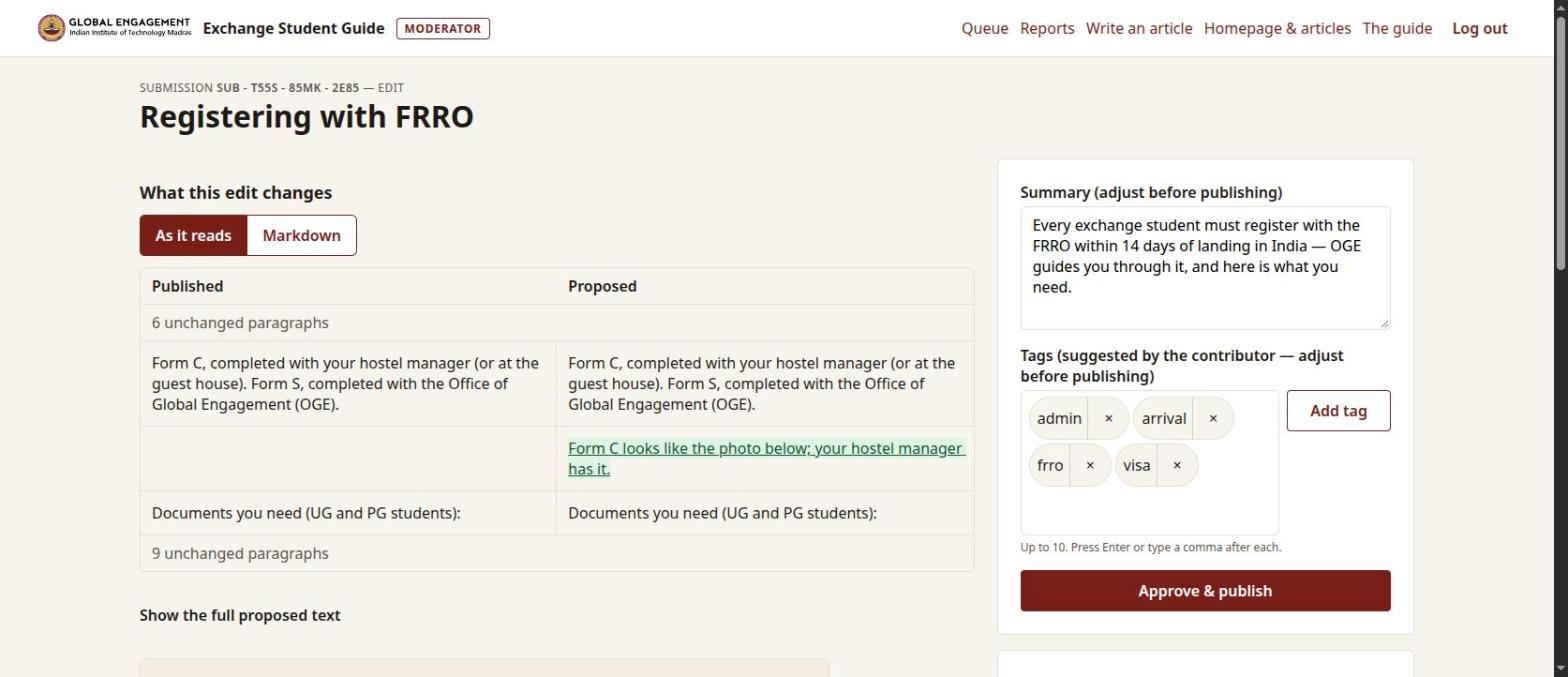
\includegraphics[height=0.8\textheight,width=\linewidth,keepaspectratio]{7-review.jpg}
\end{frame}

\begin{frame}{Backup: decisions and the options we weighed}
\small
\begin{tabularx}{\textwidth}{@{}lX@{}}
\toprule
ADR-0002 & Vertical slices in one process; Spring Modulith enforces the boundary \\
ADR-0003 & A submission is its own table: an unapproved text is never a row of \texttt{article}; a revision is a full copy \\
ADR-0004 & Search through Lucene, not the database: same engine in H2 tests and PostgreSQL \\
ADR-0009 & One shared password for OGE, not accounts --- students need none at all \\
ADR-0011 & The submission number is an unguessable token, not a sequence \\
ADR-0016 & One slice owns the links table, fed by an event in the writer's transaction \\
ADR-0022 & Tag and file fields from libraries, and the CSP they need \\
\bottomrule
\end{tabularx}
\end{frame}

\begin{frame}{Backup: the code itself draws its slices}
\centering
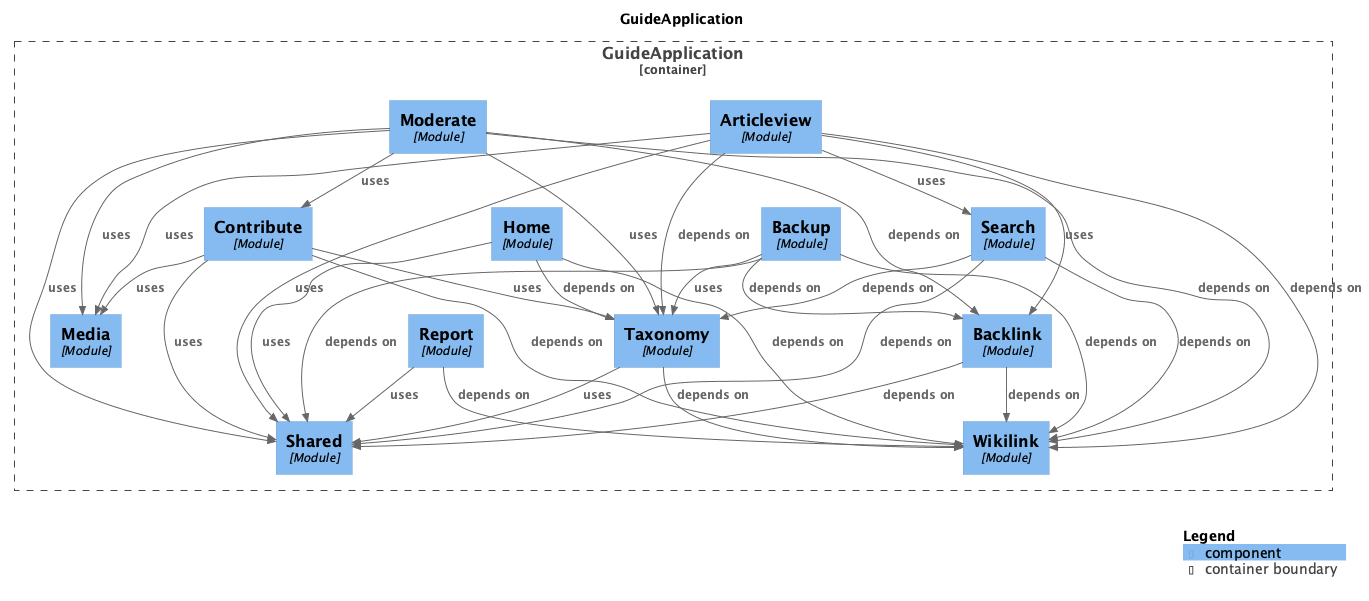
\includegraphics[height=0.8\textheight,width=\linewidth,keepaspectratio]{c4-component-actual.png}

\footnotesize Generated by Spring Modulith from the imports, in \texttt{ModularityTest}.
\end{frame}

\end{document}
